\chapter{Calculation formulas}
\label{ch2}

The purpose of this chapter is to provide the calculation formulas implemented in JPAD software and used to evaluate the aerodynamic coefficients with regard to the aircraft as a whole. The calculation formulas are mostly based on the well known USAF DATCOM~\cite{book:USAF_DATCOM}. In particular, both for the specific formulations and for the symbols, we have used a single reference, namely the textbook by Napolitano~\cite{book:Napolitano}.

In the following we will recall some of the most important formulas used to model the lateral force coefficient and the rolling and yawing moment coefficients. These assume the validity of the superposition principle and express all quantities referred to the aircraft as a sum of a number of contributions. Each aerodynamic coefficient is computed first evaluating the contribution due to each part taken singularly; then the extra contribution due to aerodynamic interferences are estimated; finally, all contributions are summed up.

From now on, all the angular gradients will be evaluated in \si{rad^{-1}}.

% --------------------------------------------------------------------------------------------------------------------------------------------
% SEZIONE 1
% --------------------------------------------------------------------------------------------------------------------------------------------
\section{Steady-state lateral force coefficient}
\label{sec2.1}

The steady-state lateral force can be evaluated by the relationship:
\begin{equation}
\label{eq:LateralForce}
Y = \CY \overline{q} \SW
\end{equation}
where the lateral force coefficient can be expressed by:
\begin{equation}
\CY = f(\beta,\deltaA,\deltaR)
\end{equation}
The first order approximation for the Taylor expansion gives the following expression for \CY:
\begin{equation}
\CY = \CYzero + \CYbeta \beta + \CYdeltaa \deltaA + \CYdeltar \deltaR
\end{equation}
in which the term \CYzero is zero if the aircraft is symmetric with respect to the \emph{XZ} plane.

% --------------------------------------------------------------------------------------------------------------------------------------------
% SOTTOSEZIONE 1.1
% --------------------------------------------------------------------------------------------------------------------------------------------
\subsection{Sideslip angle effect}
\label{subsec2.1.1}

The aerodynamic coefficient $\CYbeta$ can be expressed through its dependencies as shown in the following formula:
\begin{equation}
\label{eq:sideslipeffect1}
\CYbeta =  \CYbetaWB + \CYbetaH + \CYbetaV
\end{equation}
In this equation there are the contributions of the wing-body configuration, of the horizontal tail and of the vertical tail. For a detailed modelling of \CYbeta, it is useful to separate the contribution of the wing and of the fuselage:
\begin{equation}
\label{eq:sideslipeffect2}
\CYbeta =  \CYbetaW + \CYbetaB + \CYbetaH + \CYbetaV
\end{equation}

A relationship for the wing contribution is given by:
\begin{equation}
\label{eq:sideslipW}
\CYbetaW = -0.00573 \abs \GammaW
\end{equation}

A relationship for the fuselage contribution is instead given by:
\begin{equation}
\label{eq:sideslipB}
\CYbetaB = -2 K_{\mathrm{int}} \frac{S_{\mathrm P \rightarrow \mathrm V}}{\SW}
\end{equation}
where $k_{\mathrm{int}}$ is an interference factor calculated from figure~\vref{Kint}, whereas $S_{\mathrm P \rightarrow \mathrm V}$ is the cross section at the location of the fuselage where the flow ceases to be potential.

\begin{figure}[htbp] 
\centering
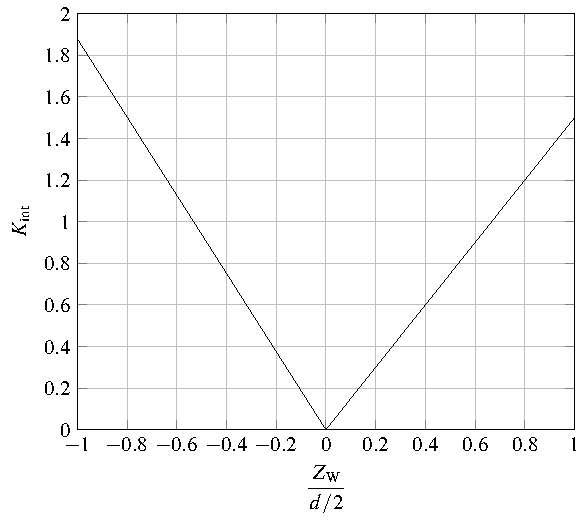
\includegraphics[width=0.75\textwidth]{Immagini/Capitolo2/4_8-Kint}
\caption[Wing-body interference factor] {Wing-body interference factor}
\label{Kint}
\end{figure}

The horizontal tail contribution is given by:
\begin{equation}
\label{eq:sideslipH}
\CYbetaH = -0.00573 \abs \GammaH \etaH \biggl( 1 - \frac{\mathrm{d}\sigma}{\mathrm{d}\beta} \biggr) \frac{\SH}{\SW}
\end{equation}

The vertical tail contribution is expressed in the following formula:
\begin{equation}
\label{eq:sideslipV}
\CYbetaV = - k_{Y_\mathrm V} \big|\CLalphaV \big| \etaV \biggl( 1 - \frac{\mathrm{d}\sigma}{\mathrm{d}\beta} \biggr) \frac{\SV}{\SW}
\end{equation}
where $k_{Y_\mathrm V}$ is an empirical factor shown in figure~\vref{KYV}.

\begin{figure}[htbp] 
\centering
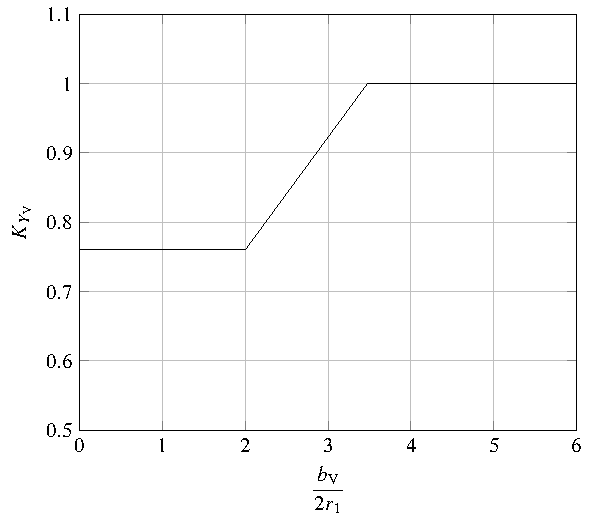
\includegraphics[width=0.75\textwidth]{Immagini/Capitolo2/4_13-KYV}
\caption[Empirical factor lateral force vertical tail due to $\beta$] {Empirical factor for the lateral force at the vertical tail due to $\beta$}
\label{KYV}
\end{figure}

% --------------------------------------------------------------------------------------------------------------------------------------------
% SOTTOSEZIONE 1.2
% --------------------------------------------------------------------------------------------------------------------------------------------
\subsection{Ailerons deflection effect}
\label{subsec2.1.2}

The ailerons are an asymmetric control surface and the forces associated with their deflections act along the vertical and horizontal directions; therefore, their components along the lateral direction is negligible. Thus, we have:
\begin{equation}
\label{eq:aileronlateralforce}
\CYdeltaa \approx 0
\end{equation}

% --------------------------------------------------------------------------------------------------------------------------------------------
% SOTTOSEZIONE 1.3
% --------------------------------------------------------------------------------------------------------------------------------------------
\subsection{Rudder deflection effect}
\label{subsec2.1.3}

The rudder is a control surface. A mathematical relationship for \CYdeltar is given by:
\begin{equation}
\label{eq:rudderlateralforce}
\CYdeltar = \big|\CLalphaV \big| \etaV \frac{\SV}{\SW} \textrm \textDelta (K_{\textrm r}) \taurud
\end{equation}
In this relationship the term \CLalphaV is the lift-curve slope for the vertical tail, $\textrm \textDelta (K_{\textrm r})$ is a correction factor associated with the span of the rudder within the span of the vertical tail, evaluated graphically from figure~\vref{KR} using $\eta$ of the inner and outer rudder station, and \taurud is a control surface effectiveness factor, calculated from figure~\vref{taurudder}.

\begin{figure}[htbp] 
\centering
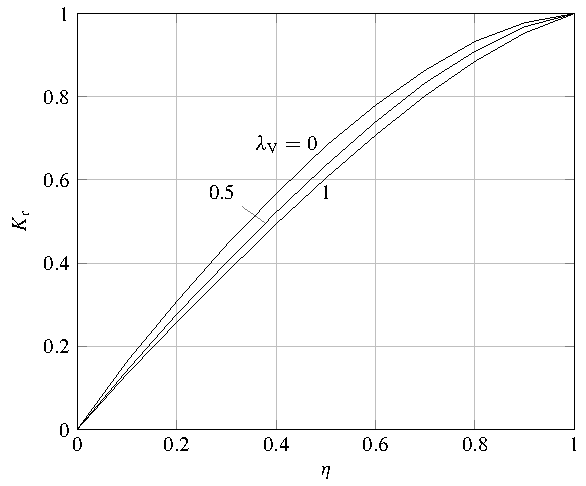
\includegraphics[width=0.75\textwidth]{Immagini/Capitolo2/4_27-KR}
\caption[Span factor rudder vertical tail] {Span factor between rudder and vertical tail}
\label{KR}
\end{figure}

\begin{figure}[htbp] 
\centering
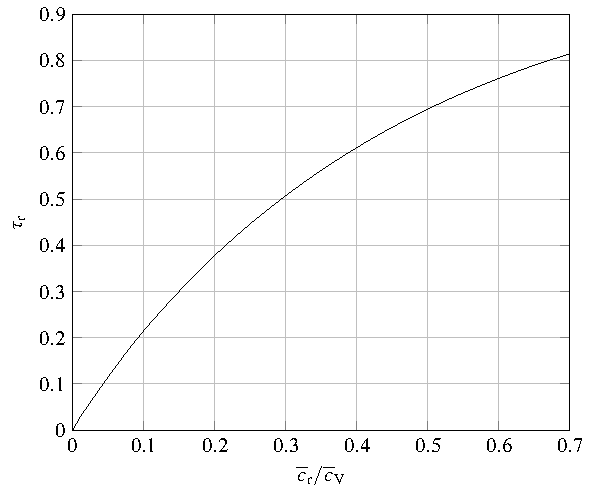
\includegraphics[width=0.75\textwidth]{Immagini/Capitolo2/4_26-Effectiveness_Rudder}
\caption[Effectiveness of the rudder] {Effectiveness of the rudder \taurud as function of $\overline c_\text r/\overline c_\text V$}
\label{taurudder}
\end{figure}

% --------------------------------------------------------------------------------------------------------------------------------------------
% SEZIONE 2
% --------------------------------------------------------------------------------------------------------------------------------------------
\newpage
\section{Steady-state rolling moment coefficient}
\label{sec2.2}

The steady-state rolling moment can be evaluated by the relationship:
\begin{equation}
\label{eq:RollMoment}
\mathcal{L} = \CL \overline{q} \SW \bW
\end{equation}
where the rolling moment coefficient can be expressed by:
\begin{equation}
\CL = f(\beta,\deltaA,\deltaR)
\end{equation}
The first order approximation for the Taylor expansion gives the following expression for \CL:
\begin{equation}
\CL = \CLzeroRoll + \CLbeta \beta + \CLdeltaa \deltaA + \CLdeltar \deltaR
\end{equation}
in which the term \CLzeroRoll is zero if the aircraft is symmetric with respect to the \emph{XZ} plane.

% --------------------------------------------------------------------------------------------------------------------------------------------
% SOTTOSEZIONE 2.1
% --------------------------------------------------------------------------------------------------------------------------------------------
\subsection{Dihedral effect}
\label{subsec2.2.1}

The aerodynamic coefficient $\CLbeta$ is known as dihedral effect and it can be expressed through its dependencies as shown in the following formula:
\begin{equation}
\label{eq:dihedraleffect}
\CLbeta =  \CLbetaWB + \CLbetaH + \CLbetaV
\end{equation}
In this equation there are the contributions of the wing-body, of the horizontal tail and of the vertical tail.

The contribution of the wing-body consists of three terms: the first one is due to the wing geometric dihedral angle; the second one is due to an aerodynamic phenomenon associated with the location of the fuselage with respect to the wing (high wing or low wing); the third one is due to the geometric wing sweep angle. A closed-form expression for the modelling for $\CLbetaWB$  is given by:
\begin{multline}
\label{eq:dihedralWB}
\CLbetaWB = 57.3 \CLift \Biggl[ \Biggl(\frac{\CLbeta} {\CLift} \Biggr)_{\Lambda_{c/2}} K_{M_\Lambda}  K_{f} + \Biggl(\frac{\CLbeta} {\CLift} \Biggr)_{AR} \Biggr] + \\ + 57.3 \Biggl\{ \GammaW\Biggl[\frac{\CLbeta}{\GammaW}  K_{M_{\Gamma}} + \frac{\textrm \textDelta \CLbeta}{\GammaW}\Biggr] + \Bigl( \textrm \textDelta \CLbeta \Bigr)_{\ZW}+ \epsW \tan\Lambda_{c/4} \Biggl( \frac{\textrm \textDelta \CLbeta}{\epsW \tan \Lambda_{c/4}} \Biggr) \Biggr\}
\end{multline}
In the formula \ref{eq:dihedralWB} there are some semi-empirical coefficients:
\begin{enumerate}
\item \label{RollLiftLamb} $\bigl({\CLbeta}/{\CLift} \bigr)_{\Lambda_{c/2}}$ is the contribution associated with the wing sweep angle;
\item \label{KappaMLamb} $K_{M_\Lambda}$ is a correction factor associated with the Mach number and the wing sweep angle;
\item \label{Kappaf} $K_{f}$ is a correction factor associated with the length of the forward portion of the fuselage;
\item \label{RollLiftAR} $\bigl({\CLbeta}/{\CLift} \bigr)_{AR}$ is the contribution associated with the wing aspect ratio;
\item \label{RollGamma} ${\CLbeta}/{\GammaW}$ is the contribution associated with the wing dihedral angle;
\item \label{KappaMGamma} $K_{M_{\Gamma}}$ is a correction factor associated with the Mach number and the wing dihedral angle;
\item \label{DeltaRollGamma} ${\textrm \textDelta \CLbeta}/{{\GammaW}}$ is a correction factor associated with the size of the fuselage;
\item \label{DeltaRollZ} $\bigl( \textrm \textDelta \CLbeta \bigr)_{\ZW}$ is a correction factor associated with the location of the fuselage with respect to the wing;
\item \label{DeltaRollEps} ${\textrm \textDelta \CLbeta}/{(\epsW \tan \Lambda_{c/4})}$ is a correction factor associated with the twist angle \epsW between the zero-lift lines of the wing sections at the tip and at the root stations.
\end{enumerate}
The terms (\ref{RollLiftLamb}), (\ref{KappaMLamb}), (\ref{Kappaf}), (\ref{RollLiftAR}), (\ref{RollGamma}), (\ref{KappaMGamma}) and (\ref{DeltaRollEps}) are are given by figure~\vref{sweepanglecontribution} to figure~\vref{twistanglecontribution}. The term (\ref{DeltaRollGamma}) is modelled using the relationship:
\begin{equation}
\frac{\textrm \textDelta \CLbeta}{{\GammaW}} = -0.0005 \ARW \biggl( \frac{\dB}{\bW} \biggr)^2
\end{equation}
The factor (\ref{DeltaRollZ}) is modelled using the relationship:
\begin{equation}
\bigl( \textrm \textDelta \CLbeta \bigr)_{\ZW} = 1.2 \sqrt{\ARW} \frac{\ZW}{\bW} \biggl( \frac{2\dB}{\bW} \biggr)
\end{equation}

\begin{figure}[htbp]
\centering
\subfloat[]
	{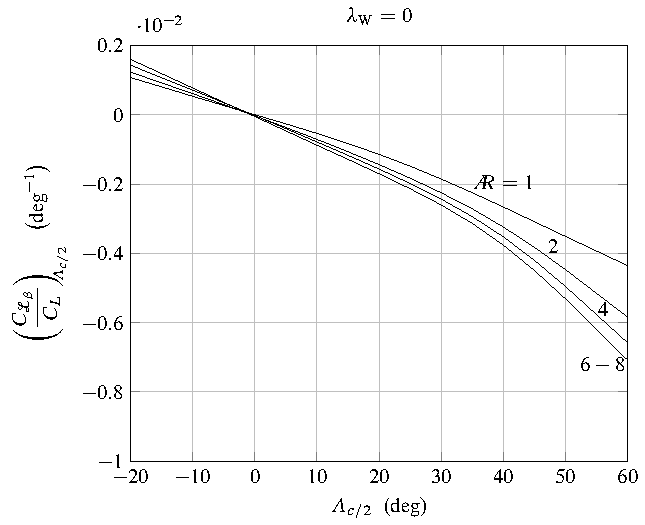
\includegraphics[width=0.55\textwidth]{Immagini/Capitolo2/4_39-K_Roll_Lam_C2_lam0}} \\
\subfloat[]
	{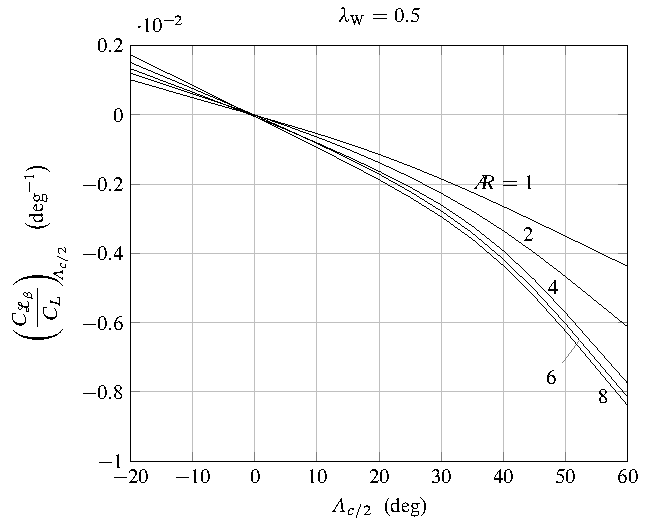
\includegraphics[width=0.55\textwidth]{Immagini/Capitolo2/4_39-K_Roll_Lam_C2_lam05}} \\
\subfloat[]
	{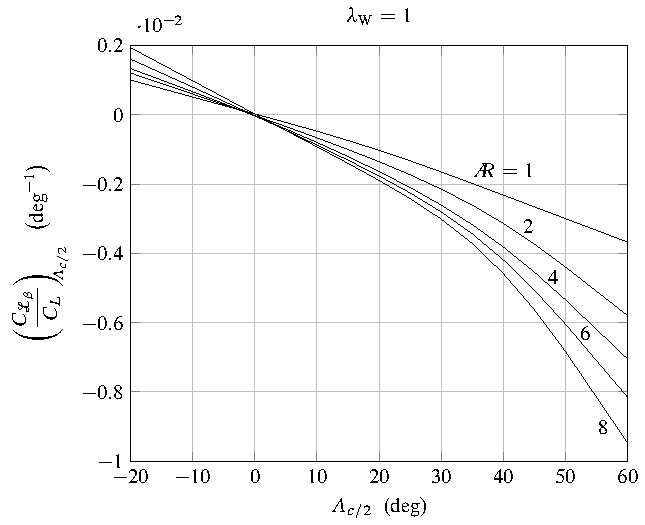
\includegraphics[width=0.55\textwidth]{Immagini/Capitolo2/4_39-K_Roll_Lam_C2_lam1}}
\caption[Contribution to \CLbetaWB due to $\Lambda_{c/2}$] {Contribution to \CLbetaWB due to wing sweep angle}
\label{sweepanglecontribution}
\end{figure}

\begin{figure}[htbp]
\centering
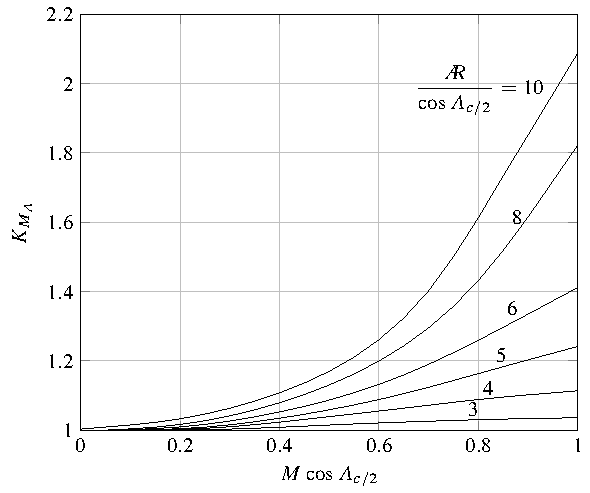
\includegraphics[width=0.55\textwidth]{Immagini/Capitolo2/4_40-K_M_Lam}
\caption[Compressibility correction factor for \CLbetaWB due to $\Lambda_{c/2}$] {Compressibility correction factor for \CLbetaWB due to wing sweep angle}
\label{compressibilitycorrection}
\end{figure}

\begin{figure}[htbp]
\centering
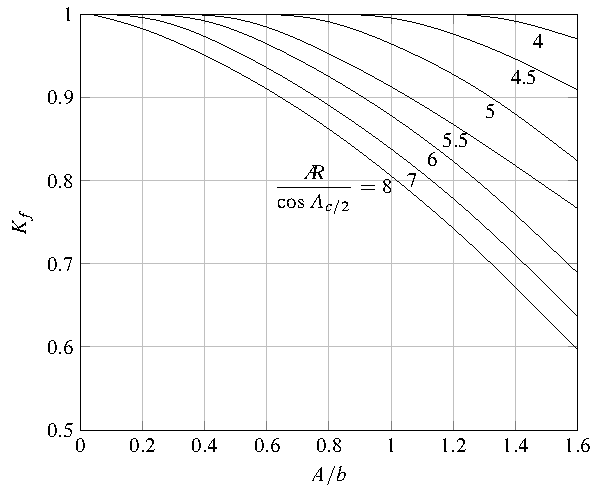
\includegraphics[width=0.55\textwidth]{Immagini/Capitolo2/4_41-K_Roll_f}
\caption[Fuselage correction factor for \CLbetaWB due to $\Lambda_{c/2}$] {Fuselage correction factor for \CLbetaWB due to wing sweep angle}
\label{fuselagecorrection}
\end{figure}

\begin{figure}[htbp]
\centering
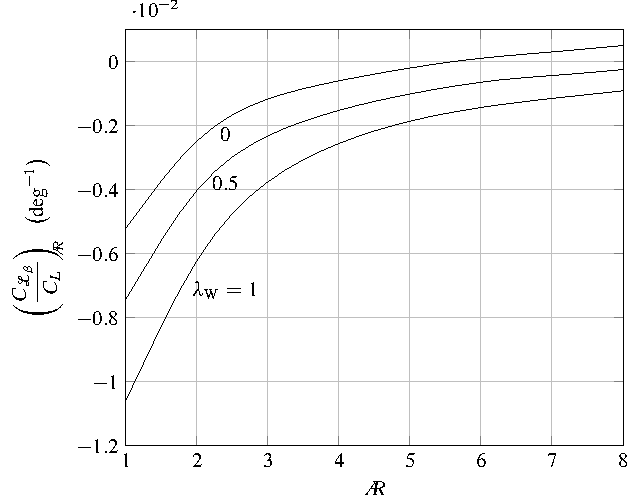
\includegraphics[width=0.55\textwidth]{Immagini/Capitolo2/4_42-K_Roll_AR}
\caption[Correction for \CLbetaWB due to \ARW] {Contribution to \CLbetaWB due to wing aspect ratio}
\label{wingaspectratiocorrection}
\end{figure}

\begin{figure}[htbp]
\centering
\subfloat[]
	{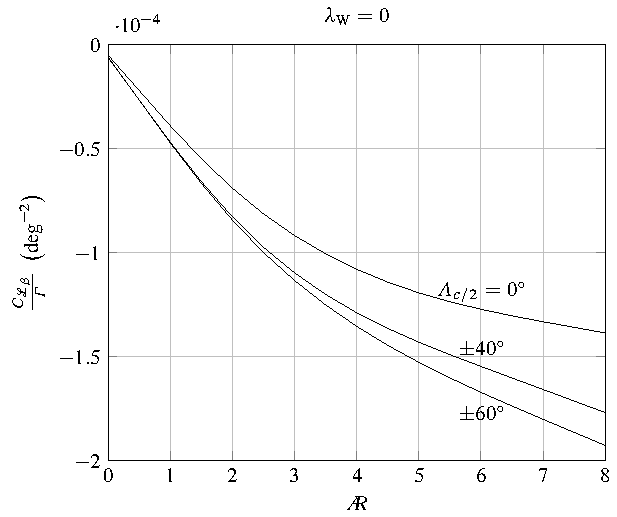
\includegraphics[width=0.55\textwidth]{Immagini/Capitolo2/4_43-K_Roll_Gam_lam0}} 
\\
\subfloat[]
	{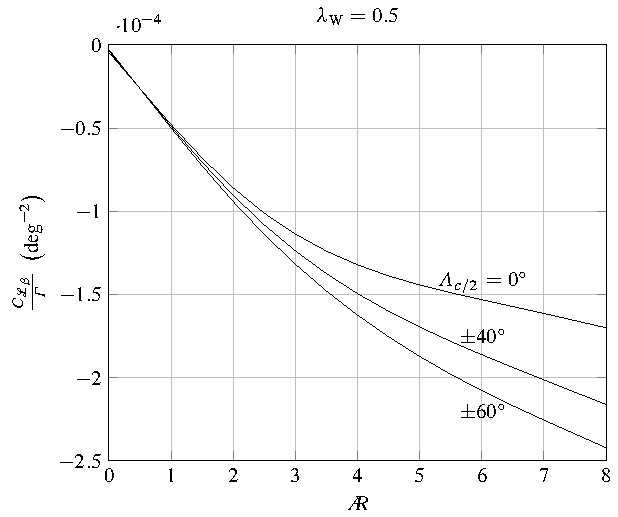
\includegraphics[width=0.55\textwidth]{Immagini/Capitolo2/4_43-K_Roll_Gam_lam05}} 
\\
\subfloat[]
	{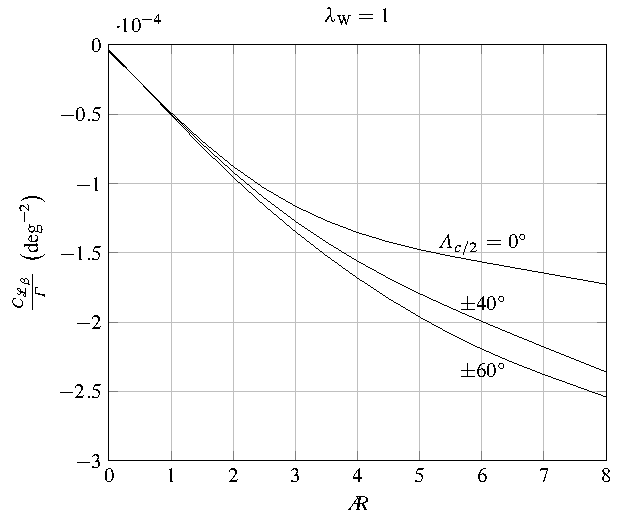
\includegraphics[width=0.55\textwidth]{Immagini/Capitolo2/4_43-K_Roll_Gam_lam1}}
\caption[Contribution to \CLbetaWB due to \GammaW] {Contribution to \CLbetaWB due to wing dihedral angle}
\label{dihedralanglecontribution}
\end{figure}

\begin{figure}[htbp]
\centering
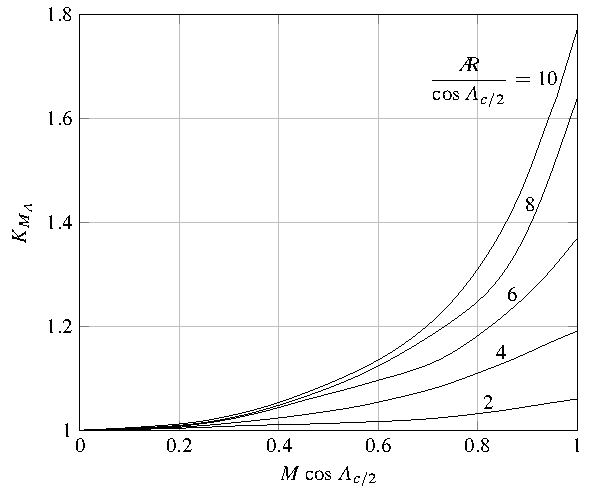
\includegraphics[width=0.75\textwidth]{Immagini/Capitolo2/4_44-K_Roll_M_Gam}
\caption[Compressibility correction factor for \CLbetaWB due to \GammaW] {Compressibility correction factor for \CLbetaWB due to wing dihedral angle}
\label{compressibilitycorrectiondihedral}
\end{figure}

\begin{figure}[htbp]
\centering
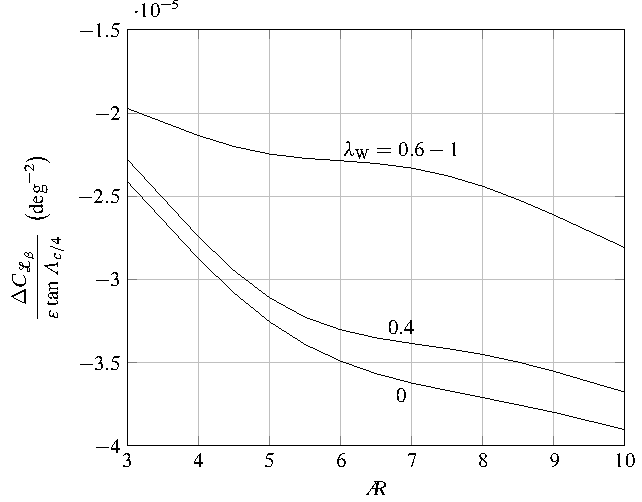
\includegraphics[width=0.75\textwidth]{Immagini/Capitolo2/4_46-K_Roll_Cl_Lam_twist}
\caption[Contribution to \CLbetaWB due to \epsW] {Contribution to \CLbetaWB due to wing twist angle}
\label{twistanglecontribution}
\end{figure}

The horizontal tail can be considered as a wing, operating at a lower dynamic pressure, with a smaller surface and a smaller span. Therefore, a relationship for \CLbetaH is given by:
\begin{equation}
\label{eq:dihedralH}
\CLbetaH = \CLbetaWB \Big|_{\mathrm H} \etaH \frac{\SH}{\SW} \frac{\bH}{\bW}
\end{equation}
where the $\CLbetaWB \big|_{\mathrm H}$ is the previously introduced \CLbetaWB evaluated with the geometric parameters of the horizontal tail. 

The vertical tail contribution to the dihedral effect is expressed by the following formula:
\begin{equation}
\label{eq:dihedralV}
\begin{split}
\CLbetaV & = \CYbetaV \frac{\ZV \cos\alphaB - \XV\sin\alphaB}{\bW} = \\
& = - k_{Y_\mathrm V} \big|\CLalphaV \big| \etaV \biggl( 1 - \frac{\mathrm{d}\sigma}{\mathrm{d}\beta} \biggr) \frac{\SV}{\SW} \frac{\ZV \cos\alphaB - \XV\sin\alphaB}{\bW}
\end{split}
\end{equation}

% --------------------------------------------------------------------------------------------------------------------------------------------
% SOTTOSEZIONE 2.2
% --------------------------------------------------------------------------------------------------------------------------------------------
\subsection{Ailerons deflection effect}
\label{subsec2.2.2}

Ailerons are an asymmetric control surface. According to European conventions, a positive deflection of the ailerons implies a trailing edge down deflection of the right aileron and a trailing edge up deflection of the left aileron. The combined result of these deflections is a negative rolling moment. The mathematical expression of $\CLdeltaa$ is:
\begin{equation}
\label{eq:ailRoll}
\CLdeltaa = \CLdeltaa' \tauail
\end{equation}
where $\CLdeltaa'$ is given by the following relationship:
\begin{equation}
\CLdeltaa' = - \textrm \textDelta (R\hspace{-0.1em} M \hspace{-0.2em} E) \frac{k}{\sqrt{1 - M^2}}
\end{equation}
in which $R \hspace{-0.1em} M \hspace{-0.2em} E$ is given by charts of figures~\vref{rme0} to~\vref{rme1}. The term \tauail is a control surface effectiveness factor, calculated from figure~\vref{tauaileron}. Finally, the term $k$ is equal to: %; in this parameter it is made the assumption that the entire wing section between the aileron inner and outer stations is deflected
\begin{equation}
k = \frac{\CLalphaW \sqrt{1 - M^2}}{2\pi}
\end{equation}

\begin{figure}[H]
\centering
\subfloat[]
	{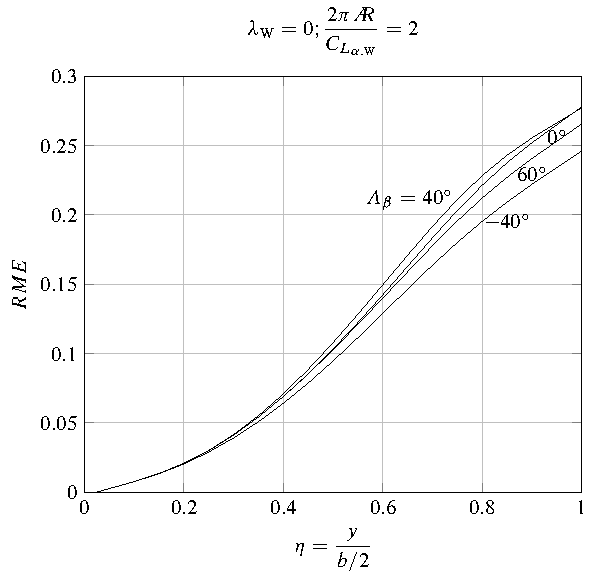
\includegraphics[width=0.5\textwidth]{Immagini/Capitolo2/4_51-RME_lam0_2}}\\
\subfloat[]
	{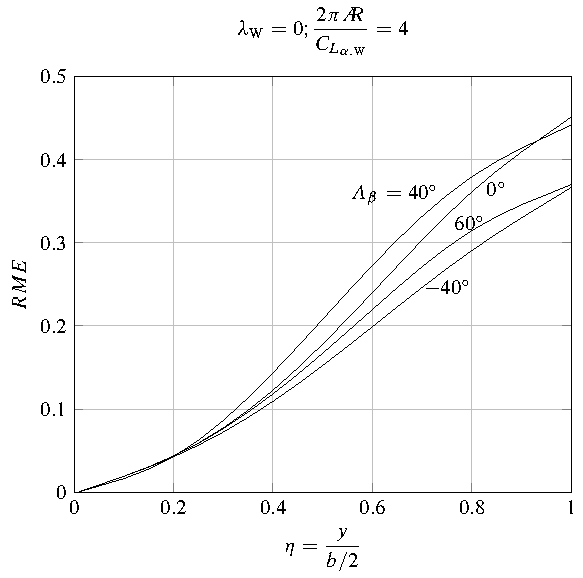
\includegraphics[width=0.5\textwidth]{Immagini/Capitolo2/4_51-RME_lam0_4}}\\
\subfloat[]
	{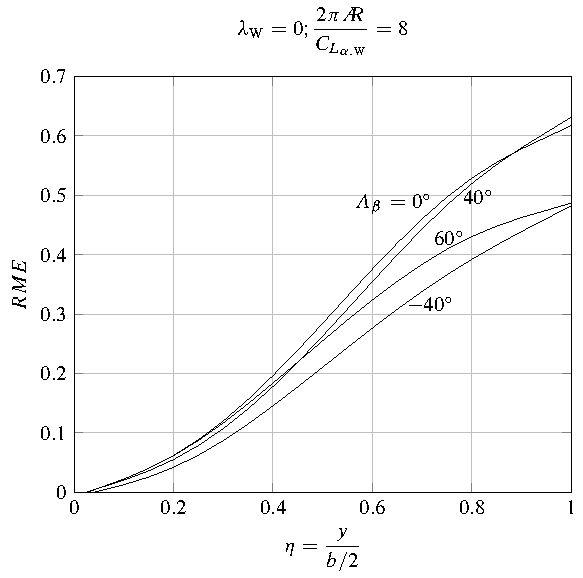
\includegraphics[width=0.5\textwidth]{Immagini/Capitolo2/4_51-RME_lam0_8}}
\caption[Rolling Moment Effectiveness for $\lambdaW = 0$] {Rolling Moment Effectiveness for different geometries of the wing ($\lambdaW = 0$)}
\label{rme0}
\end{figure}

\begin{figure}[H]
\centering
\subfloat[]
	{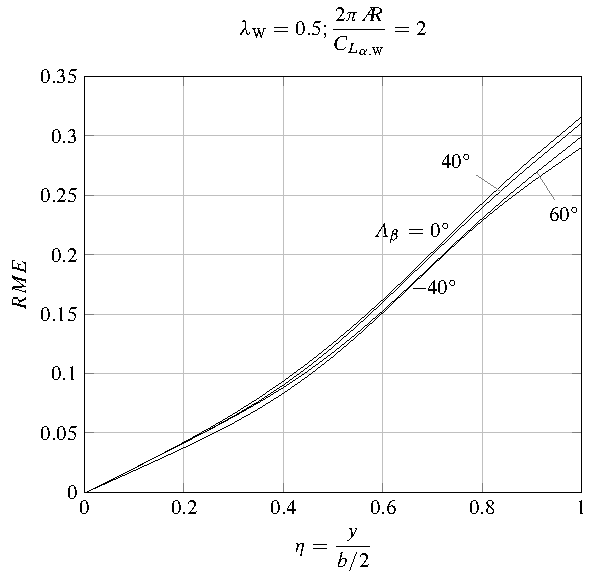
\includegraphics[width=0.5\textwidth]{Immagini/Capitolo2/4_52-RME_lam05_2}} \\
\subfloat[]
	{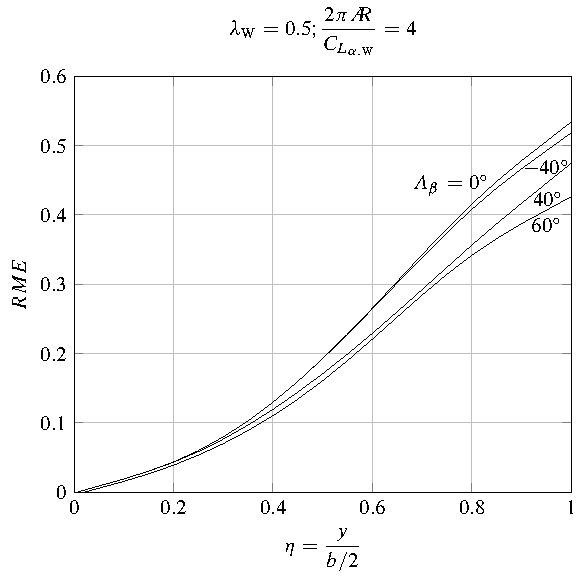
\includegraphics[width=0.5\textwidth]{Immagini/Capitolo2/4_52-RME_lam05_4}} \\
\subfloat[]
	{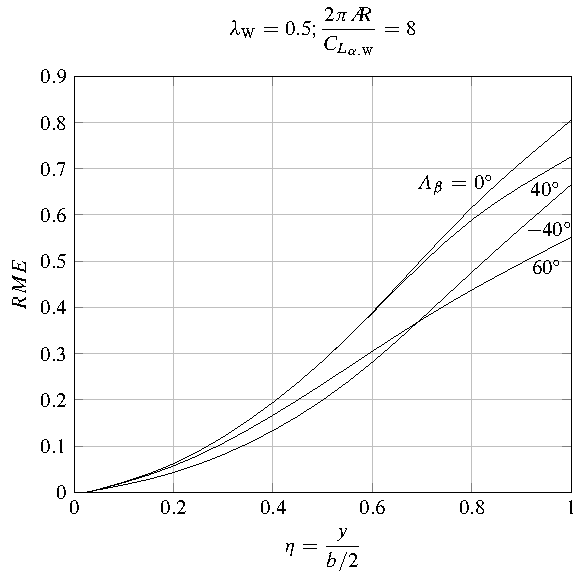
\includegraphics[width=0.5\textwidth]{Immagini/Capitolo2/4_52-RME_lam05_8}}
\caption[Rolling Moment Effectiveness for $\lambdaW = 0.5$] {Rolling Moment Effectiveness for different geometries of the wing ($\lambdaW = 0.5$)}
\label{rme05}
\end{figure}

\begin{figure}[H]
\centering
\subfloat[]
	{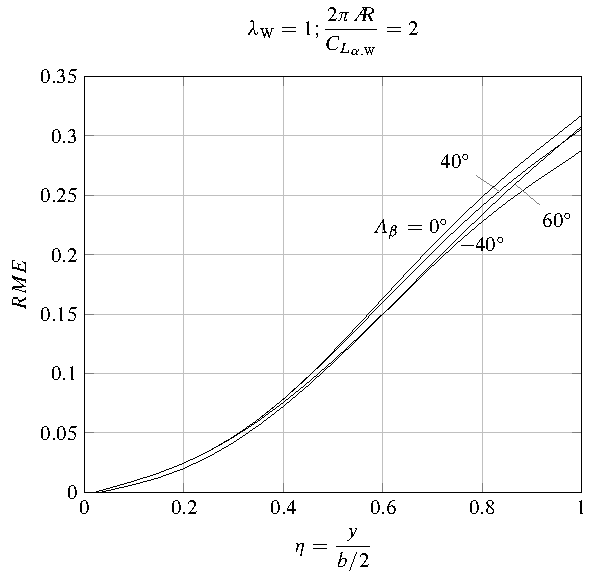
\includegraphics[width=0.5\textwidth]{Immagini/Capitolo2/4_53-RME_lam1_2}} \\
\subfloat[]
	{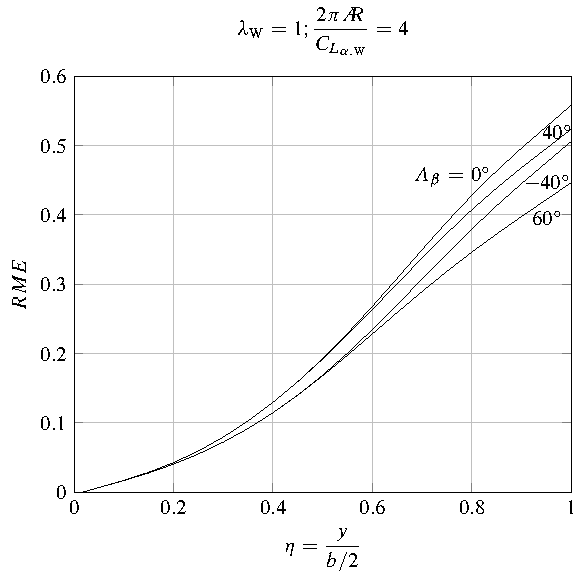
\includegraphics[width=0.5\textwidth]{Immagini/Capitolo2/4_53-RME_lam1_4}} \\
\subfloat[]
	{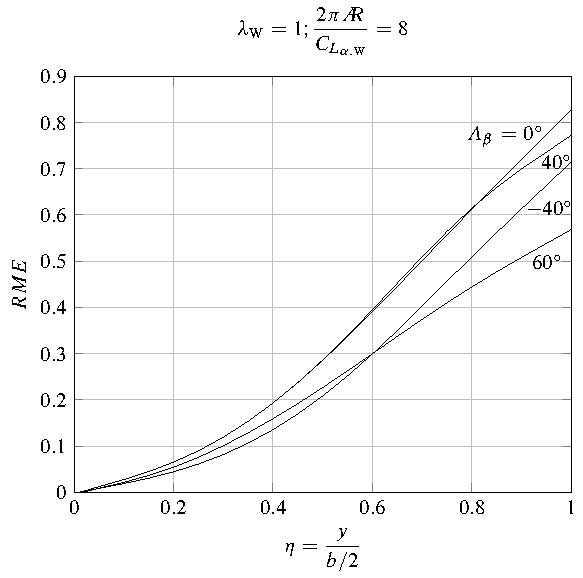
\includegraphics[width=0.5\textwidth]{Immagini/Capitolo2/4_53-RME_lam1_8}}
\caption[Rolling Moment Effectiveness for $\lambdaW = 1$] {Rolling Moment Effectiveness for different geometries of the wing ($\lambdaW = 1$)}
\label{rme1}
\end{figure}

\begin{figure}[H]
\centering
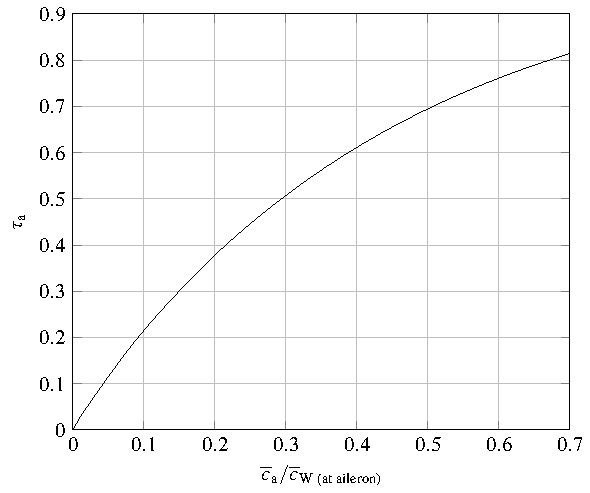
\includegraphics[width=0.75\textwidth]{Immagini/Capitolo2/4_55-Effectiveness_Aileron}
\caption[Effectiveness of the aileron] {Effectiveness of the aileron \tauail as function of $\overline c_\text a/\overline c_{\text {W (at aileron)}}$}
\label{tauaileron}
\end{figure}

% --------------------------------------------------------------------------------------------------------------------------------------------
% SOTTOSEZIONE 2.3
% --------------------------------------------------------------------------------------------------------------------------------------------
\subsection{Rudder deflection effect}
\label{subsec2.2.3}

The rudder is the control surface, hinged at the tip of the vertical tail, which provides yaw control. Its contribution to the rolling moment originates from the lateral force associated with its deflection through its moment arm with respect to the aircraft centre of gravity. A mathematical relationship for this moment coefficient is:
\begin{equation}
\label{eq:rollRudder}
\CLdeltar = \CYdeltar \frac{\ZR \cos\alphaB - \XR \sin\alphaB}{\bW} = \big|\CLalphaV \big| \etaV \frac{\SV}{\SW} \textrm \textDelta (K_{\textrm r}) \taurud \frac{\ZR \cos\alphaB - \XR \sin\alphaB}{\bW}
\end{equation}

% --------------------------------------------------------------------------------------------------------------------------------------------
% SEZIONE 3
% --------------------------------------------------------------------------------------------------------------------------------------------
\section{Steady-state yawing moment coefficient}
\label{sec2.3}

The steady-state yawing moment can be evaluated by the relationship:
\begin{equation}
\label{eq:YawMoment}
\mathcal{N} = \CN \overline{q} \SW \bW
\end{equation}
where the rolling moment coefficient can be expressed by:
\begin{equation}
\CN = f(\beta,\deltaA,\deltaR)
\end{equation}
The first order approximation for the Taylor expansion gives the following expression for \CN :
\begin{equation}
\CN = \CNzeroYaw + \CNbeta \beta + \CNdeltaa \deltaA + \CNdeltar \deltaR
\end{equation}
in which the term \CNzeroYaw is zero if the aircraft is symmetric with respect to the \emph{XZ} plane.

% --------------------------------------------------------------------------------------------------------------------------------------------
% SOTTOSEZIONE 3.1
% --------------------------------------------------------------------------------------------------------------------------------------------
\subsection{Weathercock effect}
\label{subsec2.3.1}

The aerodynamic coefficient \CNbeta is known as weathercock effect and it can be expressed through its dependencies as shown in the following formula:
\begin{equation}
\label{eq:weathercockeffect}
\CNbeta = \CNbetaW + \CNbetaBody + \CNbetaH + \CNbetaV
\end{equation}

The contribution of the wing and the horizontal tail are negligible for all configurations. 

The fuselage contribution is evaluated using the relationship:
\begin{equation}
\label{eq:weathercockBody}
\CNbetaBody = -57.3 K_{\textrm N} K_{\textrm{Re}_\textrm B} \frac{\SBside}{\SW} \frac{\lB}{\bW}
\end{equation}
where the coefficient $K_{\textrm N}$ is an empirical factor, given by figure~\vref{wingbodyinterface} and related to the geometric coefficients of the axial cross section of the fuselage, whereas the coefficient $K_{\textrm{Re}_\textrm B}$, given by figure~\vref{reynoldscontribution}, is related to the fuselage Reynolds number.

The most significant contribution to \CNbeta is provided by the vertical tail. This contribution is evaluated by:
\begin{equation}
\label{eq:weathercockVertical}
\begin{split}
\CNbetaV & = -\CYbetaV \frac{\ZV \sin\alphaB + \XV \cos\alphaB}{\bW} = \\
& = k_{Y_\textrm V} \big|\CLalphaV \big| \etaV \biggl( 1 - \frac{\mathrm{d}\sigma}{\mathrm{d}\beta} \biggr) \frac{\SV}{\SW} \frac{\ZV \sin\alphaB + \XV \cos\alphaB}{\bW}
\end{split}
\end{equation}

\begin{figure}[htbp]
\centering
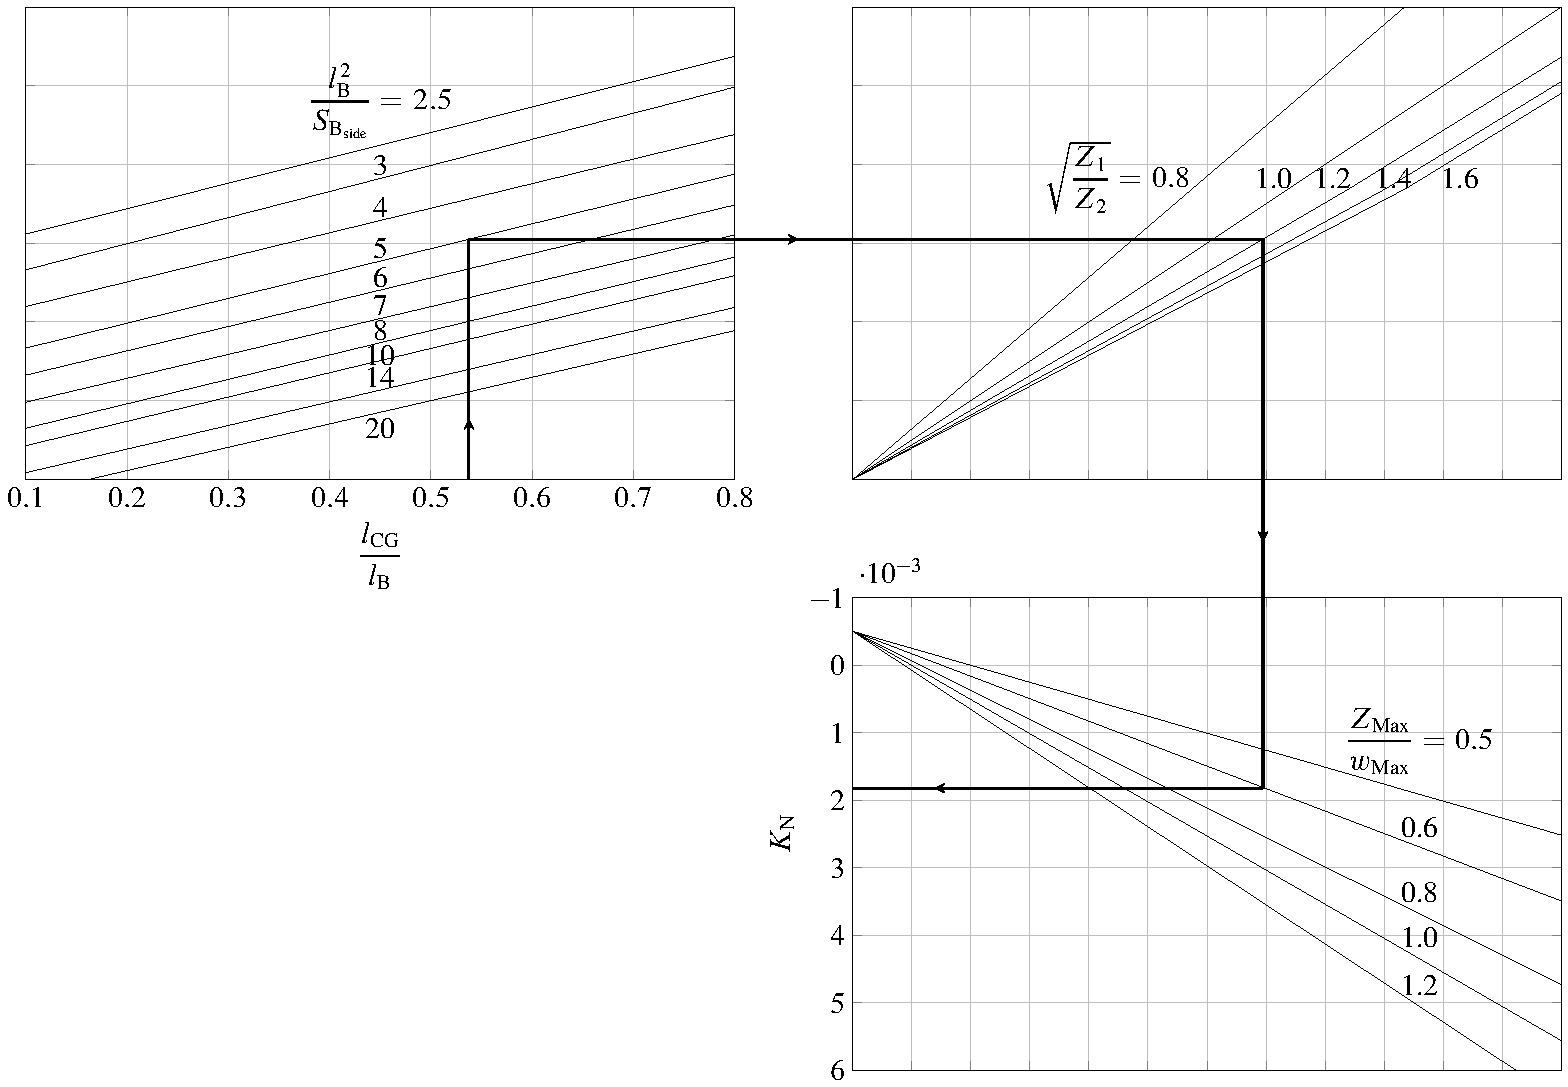
\includegraphics[width=\textwidth]{Immagini/Capitolo2/4_68-KN}
\caption[Empirical factor $K_\text N$ for wing-body interface] {Empirical factor $K_\text N$ for wing-body interface}
\label{wingbodyinterface}
\end{figure}

\begin{figure}[htbp]
\centering
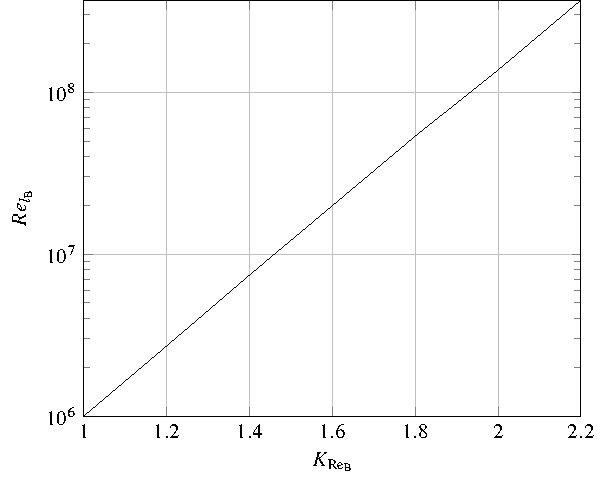
\includegraphics[width=0.75\textwidth]{Immagini/Capitolo2/4_69-KReB}
\caption[Effect of Reynolds number on wing-body interface] {Effect of Reynolds number on wing-body interface}
\label{reynoldscontribution}
\end{figure}

% --------------------------------------------------------------------------------------------------------------------------------------------
% SOTTOSEZIONE 3.2
% --------------------------------------------------------------------------------------------------------------------------------------------
\subsection{Ailerons deflection effect}
\label{subsec2.3.2}

The asymmetric deflection of the left and right ailerons also generate small but not negligible drag force leading to a small positive yawing moment. A relationship for modelling \CNdeltaa is given by:
\begin{equation}
\label{eq:yawailerons}
\CNdeltaa = - \textrm \textDelta \bigl(K_{\mathcal{N}_\textrm a} \bigr) \CLift \CLdeltaa
\end{equation}
where \CLift is the aircraft lift coefficient, the term \CLdeltaa is the rolling moment coefficient due to ailerons deflection and $K_{\mathcal{N}_\textrm a}$ is evaluated from graphs of figure~\vref{aileroncontribution}.

\begin{figure}[htbp]
\subfloat[]
	{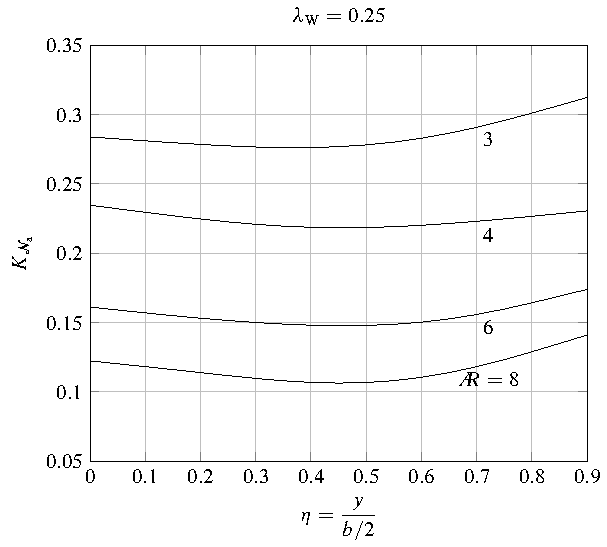
\includegraphics[width=.5\textwidth]{Immagini/Capitolo2/4_72-KNA_vs_eta_lam025}}
\subfloat[]
	{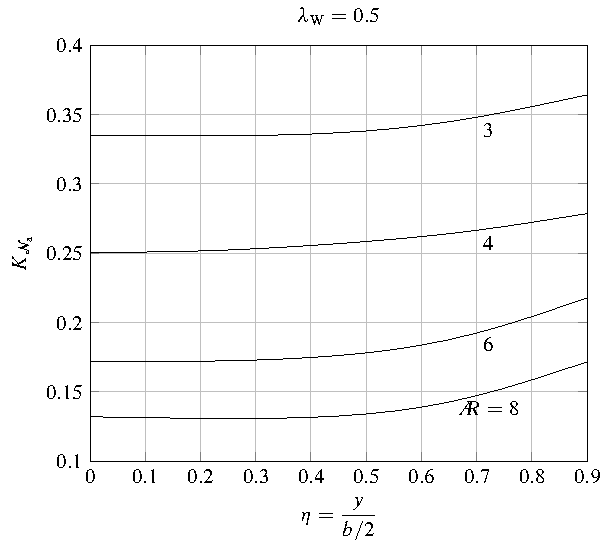
\includegraphics[width=.5\textwidth]{Immagini/Capitolo2/4_72-KNA_vs_eta_lam05}} \\
\subfloat[]
	{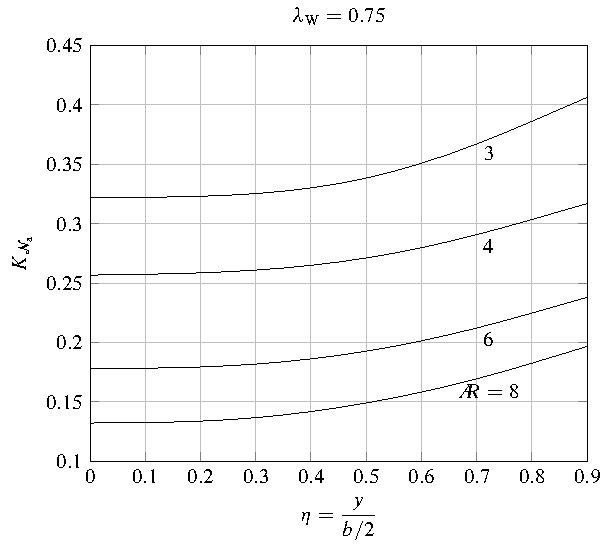
\includegraphics[width=.5\textwidth]{Immagini/Capitolo2/4_72-KNA_vs_eta_lam075}}
\subfloat[]
	{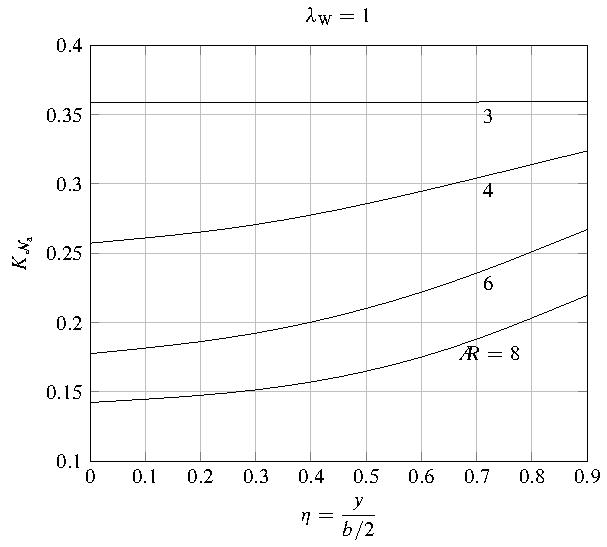
\includegraphics[width=.5\textwidth]{Immagini/Capitolo2/4_72-KNA_vs_eta_lam1}}
\caption[Correlation coefficient for $\mathcal N$ due to $\delta_\text a$] {Correlation coefficient for yawing moment due to deflection of ailerons}
\label{aileroncontribution}
\end{figure}

% --------------------------------------------------------------------------------------------------------------------------------------------
% SOTTOSEZIONE 3.3
% --------------------------------------------------------------------------------------------------------------------------------------------
\subsection{Rudder deflection effect}
\label{subsec2.3.3}

This coefficient is related to the contribution given by the rudder deflection. The mathematical expression is: 
\begin{equation}
\label{eq:yawrudder}
\begin{split}
\CNdeltar & = -\CYdeltar \frac{\ZR\sin\alphaB + \XR \cos\alphaB}{\bW} = \\
& = - \big|\CLalphaV \big| \etaV \frac{\SV}{\SW} \textrm \textDelta (K_{\textrm r}) \taurud \frac{\ZR\sin\alphaB + \XR \cos\alphaB}{\bW}
\end{split}
\end{equation}

% --------------------------------------------------------------------------------------------------------------------------------------------
% SEZIONE 4
% --------------------------------------------------------------------------------------------------------------------------------------------
\newpage
\section{Unsteady-state lateral force coefficient}
\label{sec2.4}

% --------------------------------------------------------------------------------------------------------------------------------------------
% SOTTOSEZIONE 4.1
% --------------------------------------------------------------------------------------------------------------------------------------------
\subsection{Roll rate effect}
\label{subsec2.4.1}

The coefficient \CYprate models the contribution of the lateral force coefficient due to roll rate. The vertical tail is the only component of the aircraft contributing to \CYprate. The mathematical relationship is given by:
\begin{equation}
\label{eq:sideforcerollrate}
\begin{split}
\CYprate \approx \CYprateV & = 2 \CYbetaV \frac{\ZV \cos\alphaB - \XV\sin\alphaB}{\bW} = \\
& = -2 k_{Y_\textrm V} \big|\CLalphaV \big| \etaV \biggl( 1 - \frac{\mathrm{d}\sigma}{\mathrm{d}\beta} \biggr) \frac{\SV}{\SW} \frac{\ZV \cos\alphaB - \XV\sin\alphaB}{\bW}
\end{split}
\end{equation}

% --------------------------------------------------------------------------------------------------------------------------------------------
% SOTTOSEZIONE 4.2
% --------------------------------------------------------------------------------------------------------------------------------------------
\subsection{Yaw rate effect}
\label{subsec2.4.2}

The coefficient \CYrrate models the contribution of the lateral force coefficient due to yaw rate. As for \CYprate, the vertical tail is the only component of the aircraft contributing to \CYrrate. The mathematical relationship is given by:
\begin{equation}
\label{eq:sideforceyawrate}
\begin{split}
\CYrrate \approx \CYrrateV & = - 2 \CYbetaV \frac{\ZV\sin\alphaB + \XV \cos\alphaB}{\bW} = \\
& = 2 k_{Y_\textrm V} \big|\CLalphaV \big| \etaV \biggl( 1 - \frac{\mathrm{d}\sigma}{\mathrm{d}\beta} \biggr) \frac{\SV}{\SW} \frac{\ZV\sin\alphaB + \XV \cos\alphaB}{\bW}
\end{split}
\end{equation}

% --------------------------------------------------------------------------------------------------------------------------------------------
% SEZIONE 5
% --------------------------------------------------------------------------------------------------------------------------------------------
\section{Unsteady-state rolling moment coefficient}
\label{sec2.5}

% --------------------------------------------------------------------------------------------------------------------------------------------
% SOTTOSEZIONE 5.1
% --------------------------------------------------------------------------------------------------------------------------------------------
\subsection{Roll rate effect}
\label{subsec2.5.1}

The coefficient \CLprate models the contribution of the rolling moment coefficient due to roll rate. The mathematical relationship is given by:
\begin{equation}
\label{eq:rollrollrate}
\CLprate = \CLprateWB + \CLprateH + \CLprateV
\end{equation}

The contribution of the fuselage is negligible, so $\CLprateWB \approx \CLprateW$, and the relationship for this coefficient is given by:
\begin{equation}
\label{eq:rollrollrateW}
\CLprateW = RDP \frac{k}{\sqrt{1 - M^2}}
\end{equation}
where \emph{RDP} is the rolling damping parameter, evaluated from graphs of figure~\vref{rollingdampingparameters}.

\begin{figure}[H] 
\centering
\subfloat[]
	{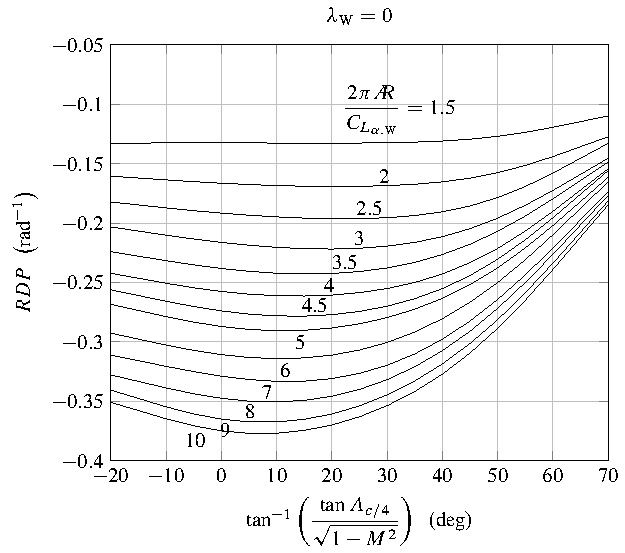
\includegraphics[width=.5\textwidth]{Immagini/Capitolo2/4_80-RDP_lam0}}
\subfloat[]
	{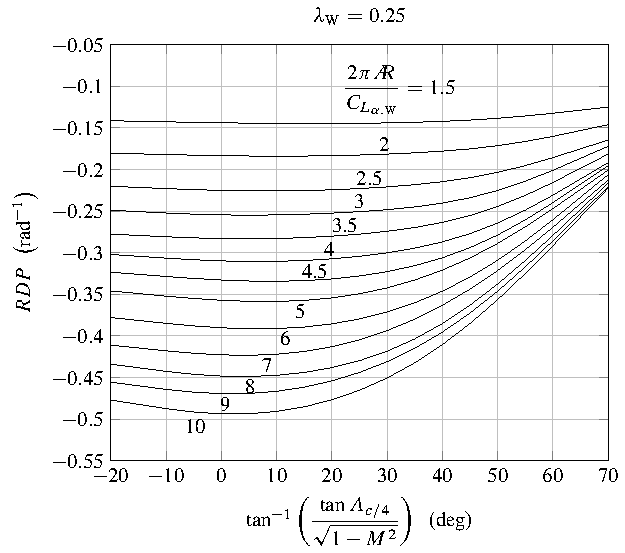
\includegraphics[width=.5\textwidth]{Immagini/Capitolo2/4_80-RDP_lam025}} \\
\subfloat[]
	{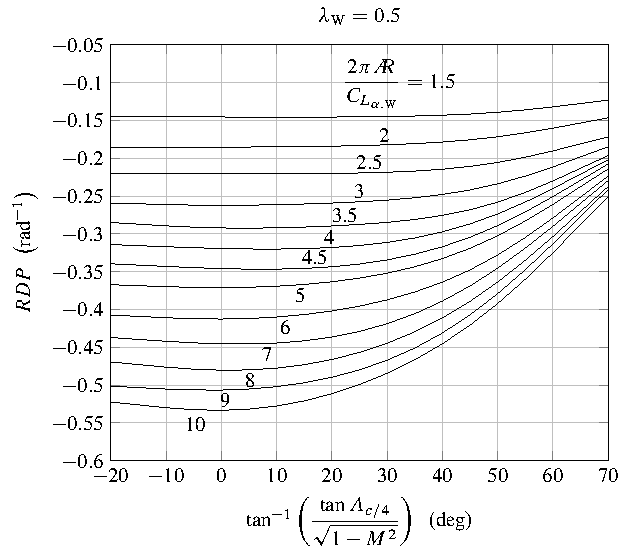
\includegraphics[width=.5\textwidth]{Immagini/Capitolo2/4_81-RDP_lam05}}
\subfloat[]
	{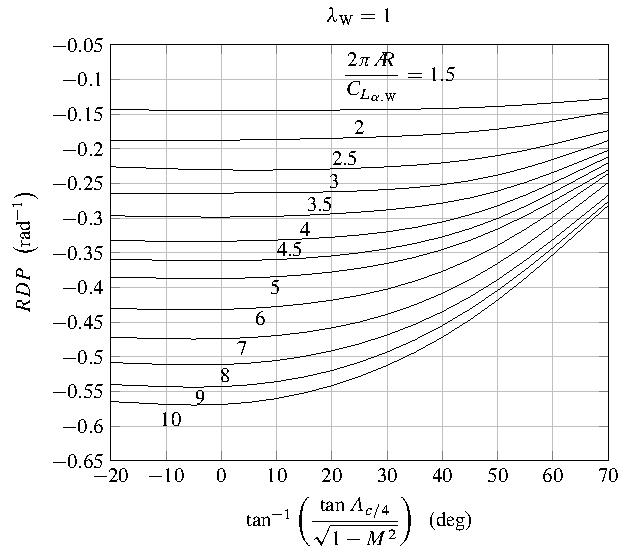
\includegraphics[width=.5\textwidth]{Immagini/Capitolo2/4_81-RDP_lam1}}
\caption[Rolling Damping Parameters] {Rolling Damping Parameters for different wing geometry}
\label{rollingdampingparameters}
\end{figure}

A relationship for \CLprateH is given by:
\begin{equation}
\label{eq:rollrollrateH}
\CLprateH = \frac{1}{2} \CLprateW \Big|_{\textrm H} \frac{\SH}{\SW} \biggl( \frac{\bH}{\bW} \biggr)^2
\end{equation}
where the $\CLprateW \big|_{\textrm  H}$ is the previously introduced \CLprateW evaluated with the geometric parameters of the horizontal tail. This coefficient is often negligible due to the low numerical value of the product of $\SH / \SW \cdot (\bH / \bW)^2$.

The contribution of the vertical tail is:
\begin{equation}
\label{eq:rollrollrateV}
\CLprateV = 2 \CYbetaV \biggl( \frac{\ZV}{\bW} \biggr)^2 = - 2  k_{Y_\textrm V}  \big|\CLalphaV \big| \etaV \biggl( 1 - \frac{\mathrm{d}\sigma}{\mathrm{d}\beta} \biggr) \frac{\SV}{\SW} \biggl( \frac{\ZV}{\bW} \biggr)^2
\end{equation}

% --------------------------------------------------------------------------------------------------------------------------------------------
% SOTTOSEZIONE 5.2
% --------------------------------------------------------------------------------------------------------------------------------------------
\subsection{Yaw rate effect}
\label{subsec2.5.2}

The contribution to the rolling moment due to the yaw rate is contained in the coefficient \CLrrate. The modelling for this coefficient starts from the following relationship:
\begin{equation}
\label{eq:rollyawrate}
\CLrrate = \CLrrateWB + \CLrrateH + \CLrrateV
\end{equation}
The fuselage and the horizontal tail do not significantly contribute to this coefficient, so we have $\CLrrate \approx \CLrrateW + \CLrrateV$.

The wing contribution is given by:
\begin{equation}
\label{eq:rollyawrateW}
\CLrrateW = \Biggl( \frac{\CLrrate}{\CLift} \Biggr) \Bigg|_{\CLift = 0} \CLift + \Biggl( \frac{\textrm \textDelta\CLrrate}{\GammaW} \Biggr) \GammaW + \Biggl( \frac{\textrm \textDelta\CLrrate}{\epsW} \Biggr) \epsW
\end{equation}
The coefficient $\Bigl( {\CLrrate}/{\CLift} \Bigr) \Big|_{\CLift = 0}$ is given by:
\begin{equation}
\Biggl( \frac{\CLrrate}{\CLift} \Biggr) \Bigg|_{\CLift = 0} = D \Biggl( \frac{\CLrrate}{\CLift} \Biggr) \Bigg|_{M = 0, \CLift = 0}
\end{equation}
where:
\begin{equation}
D = \frac{1 + \dfrac{\ARW \bigl (1 - B^2 \bigr )}{2B \bigl [\ARW B + 2\cos\LambdaQC \bigr ]} + \dfrac{\ARW B + 2\cos\LambdaQC}{\ARW B + 4\cos\LambdaQC} \dfrac{\tan^2\LambdaQC}{8}}{1 + \dfrac{\ARW + 2\cos\LambdaQC}{\ARW + 4\cos\LambdaQC}\dfrac{\tan^2\LambdaQC}{8}}
\end{equation}
in which:
\begin{equation}
B = \sqrt{1 - M^2 \cos^2\LambdaQC}
\end{equation}
and $\Bigl( {\CLrrate}/{\CLift} \Bigr) \Big|_{M = 0, \CLift = 0}$ is given by figure~\vref{CLR}. In the equation \ref{eq:rollyawrateW} the term ${\textrm \textDelta\CLrrate}/{\GammaW}$ is a factor due to the wing dihedral angle, whereas the term ${\textrm \textDelta\CLrrate}/{\epsW}$ is a factor due to the wing twist angle. The first factor is modelled using the relationship:
\begin{equation}
\frac{\textrm \textDelta\CLrrate}{\GammaW} = \frac{1}{12} \frac{\pi \ARW \sin\LambdaQC}{\ARW + 4\cos\LambdaQC}
\end{equation}
the second one is evaluated using figure~\vref{effectwingtwistonlateralforce}.

The vertical tail contribution into the equation~\ref{eq:rollyawrate} is given by:
\begin{equation}
\label{eq:rollyawrateV}
\begin{split}
\CLrrateV & = - 2 \CYbetaV \frac{\ZV \sin\alphaB + \XV\cos\alphaB}{\bW} \frac{\ZV \cos\alphaB - \XV\sin\alphaB}{\bW} = \\
& = 2 k_{Y_\textrm V} \big|\CLalphaV \big| \etaV \biggl( 1 - \frac{\mathrm{d}\sigma}{\mathrm{d}\beta} \biggr) \frac{\SV}{\SW} \frac{\ZV \sin\alphaB + \XV\cos\alphaB}{\bW} \frac{\ZV \cos\alphaB - \XV\sin\alphaB}{\bW}
\end{split}
\end{equation}

\begin{figure}[p] 
\centering
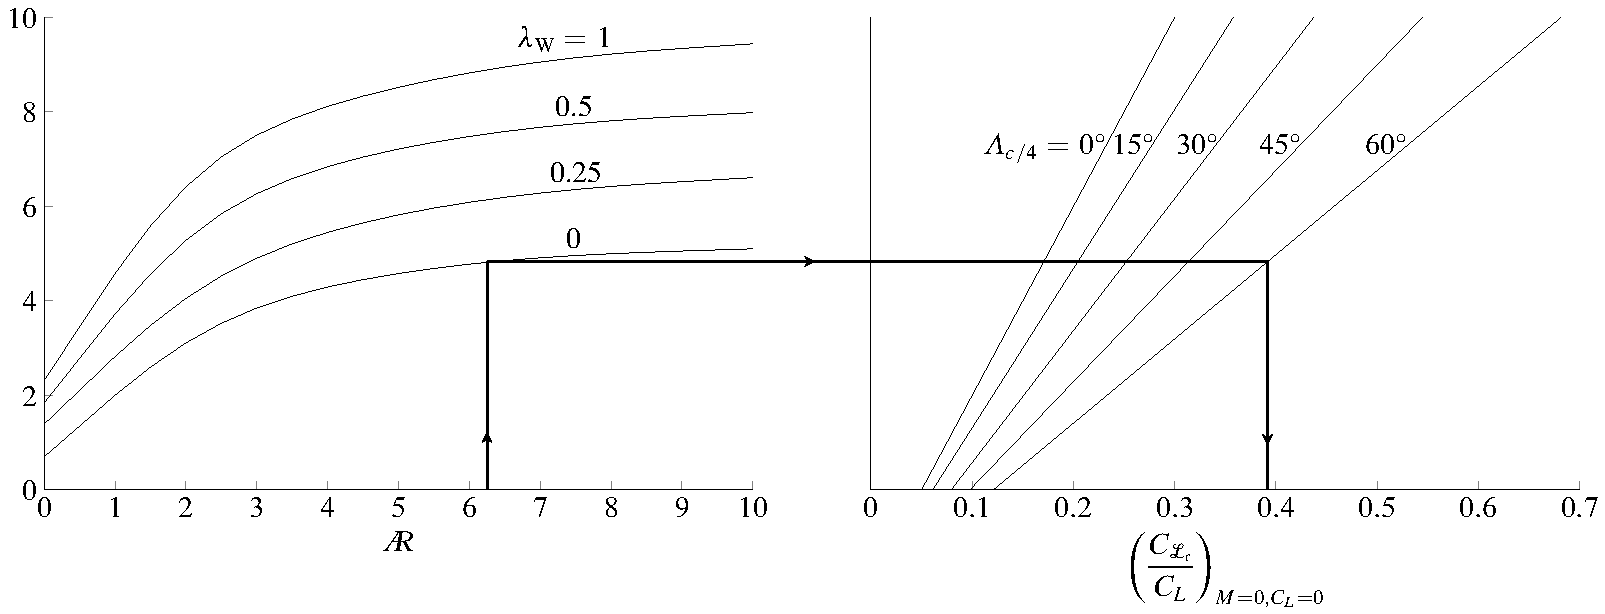
\includegraphics[width=\textwidth]{Immagini/Capitolo2/4_85-CLR}
\caption[Evaluation of $(C_{\mathcal L_{\mathrm r}}/C_L)_{M=0,C_L=0}$ ] {Evaluation of $\left(\dfrac{C_{\mathcal L_r}}{C_L}\right)_{M=0, C_L=0}$}
\label{CLR}
\end{figure}

\begin{figure}[p] 
\centering
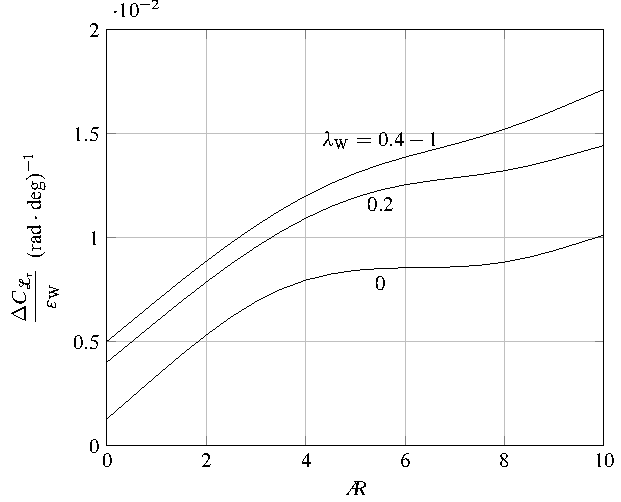
\includegraphics[width=.75\textwidth]{Immagini/Capitolo2/4_87-TwistEffect}
\caption[Effect of $\epsilon_\text W$ on $C_{\mathcal L_\mathrm r}$] {Effect of wing twist on $C_{\mathcal L_r}$.}
\label{effectwingtwistonlateralforce}
\end{figure}

% --------------------------------------------------------------------------------------------------------------------------------------------
% SEZIONE 6
% --------------------------------------------------------------------------------------------------------------------------------------------
\section{Unsteady-state yawing moment coefficient}
\label{sec2.6}

% --------------------------------------------------------------------------------------------------------------------------------------------
% SOTTOSEZIONE 6.1
% --------------------------------------------------------------------------------------------------------------------------------------------
\subsection{Roll rate effect}
\label{subsec2.6.1}

The coefficient \CNprate models the contribution to the yawing moment due to the roll rate. The relationship for this coefficient is:
\begin{equation}
\label{eq:yawrollrate}
\CNprate = \CNprateWB + \CNprateH + \CNprateV
\end{equation}
Because the fuselage and the horizontal tail do not significantly contribute to this coefficient, we have that $\CNprate \approx \CNprateW + \CNprateV$.

A relationship for the wing contribution is given by:
\begin{equation}
\label{eq:yawrollrateW}
\CNprateW = -\CLprateW \tan \alphaB + \CLprate \tan \alphaB + \Biggl( \frac{\CNprate}{\CLift} \Biggr) \Bigg|_{\CLift = 0} \CLift + \Biggl( \frac{\textrm \textDelta\CNprate}{\epsW} \Biggr) \epsW
\end{equation}
where \CLprateW and \CLprate are described in \ref{eq:rollrollrateW} and \ref{eq:rollrollrate}, respectively. The coefficient $\Bigl( {\CNprate}/{\CLift} \Bigr) \Big|_{\CLift = 0}$ is given by: 
\begin{equation}
\Biggl( \frac{\CNprate}{\CLift} \Biggr) \Bigg|_{\CLift = 0} = C \Biggl( \frac{\CNprate}{\CLift} \Biggr) \Bigg|_{M = 0, \CLift = 0}
\end{equation}
where:
\begin{equation}
C = \frac{\ARW + 4\cos\LambdaQC}{\ARW B + 4\cos\LambdaQC} \frac{\ARW B + \frac{1}{2} \bigl [\ARW B + 4\cos\LambdaQC \bigr ] \tan^2\LambdaQC}{\ARW + \frac{1}{2} \bigl [\ARW + 4\cos\LambdaQC \bigr ] \tan^2\LambdaQC}
\end{equation}
in which:
\begin{equation}
B = \sqrt{1 - M^2 \cos^2\LambdaQC}
\end{equation}
and $\Bigl ( \CNprate / \CLift \Bigr ) \Big|_{M = 0, \CLift = 0}$ is modelled using the relationship:
\begin{equation}
\Biggl( \frac{\CNprate}{\CLift} \Biggr) \Bigg|_{M = 0, \CLift = 0} = - \frac{1}{6} \frac{\ARW + 6 \bigl (\ARW + \cos\LambdaQC \bigr ) \Bigl[ (\xcgadim - \xacadim)\frac{\tan\LambdaQC}{\ARW} + \frac{\tan^2\LambdaQC}{12} \Bigr]}{\ARW + \cos\LambdaQC}
\end{equation}
The term ${\textrm \textDelta\CNprate}/{\epsW}$ is associated with the wing twist angle and is taken from figure~\vref{effectwingtwist}.

The vertical tail contribution into the equation \ref{eq:yawrollrate} is given by:
\begin{equation}
\label{eq:rollyawrateV}
\begin{split}
\CLrrateV & = -2 \CYbetaV \frac{\ZV\sin\alphaB + \XV \cos\alphaB}{\bW} \frac{\ZV \cos\alphaB - \XV\sin\alphaB - \ZV}{\bW} = \\
& = 2 k_{Y_\textrm V} \big|\CLalphaV \big| \etaV \biggl( 1 - \frac{\mathrm{d}\sigma}{\mathrm{d}\beta} \biggr) \frac{\SV}{\SW} \frac{\ZV\sin\alphaB + \XV \cos\alphaB}{\bW} \frac{\ZV \cos\alphaB - \XV\sin\alphaB - \ZV}{\bW}
\end{split}
\end{equation}

\begin{figure}[htbp]
\centering
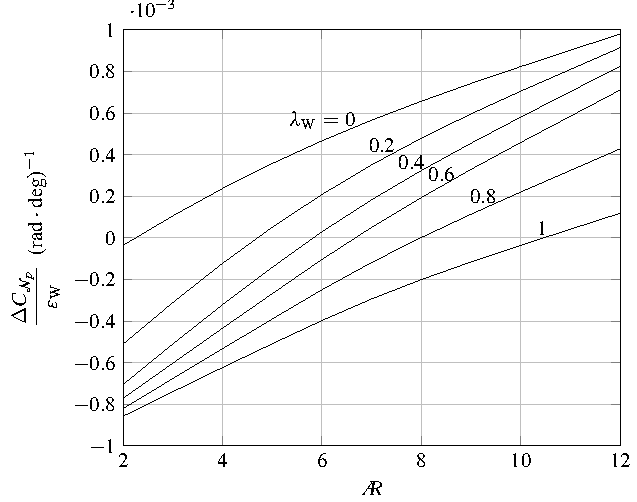
\includegraphics[width=.75\textwidth]{Immagini/Capitolo2/4_83-WingTwist_Unsteady}
\caption[Effect of wing twist on $C_{\mathcal N_\mathrm p}$] {Effect of wing twist on $C_{\mathcal N_p}$}
\label{effectwingtwist}
\end{figure}

% --------------------------------------------------------------------------------------------------------------------------------------------
% SOTTOSEZIONE 6.2
% --------------------------------------------------------------------------------------------------------------------------------------------
\subsection{Yaw rate effect}
\label{subsec2.6.2}

The coefficient \CNrrate models the contribution to the yawing moment due to the yaw rate. A relationship for this coefficient is:
\begin{equation}
\label{eq:yawyawrate}
\CNrrate = \CNrrateWB + \CNrrateH + \CNrrateV
\end{equation}
The fuselage and the horizontal tail do not significantly contribute to this coefficient; therefore, we have that $\CNrrate \approx \CNrrateW + \CNrrateV$.

The wing contribution is evaluated by the relationship:
\begin{equation}
\label{eq:yawyawrateW}
\CNrrateW = \Biggl( \frac{\CNrrate}{\CLift^2} \Biggr) \CLift^2 + \Biggl( \frac{\CNrrate}{\CDo} \Biggr) \CDo
\end{equation}
in which the terms ${\CNrrate}/{\CLift^2}$ and ${\CNrrate}/{\CDo}$ are evaluated from figure~\vref{CNR} and figure~\vref{CND} respectively.

The vertical tail contribution is given by:
\begin{equation}
\label{eq:yawyawrateV}
\begin{split}
\CNrrateV & = 2 \CYbetaV \biggl ( \frac{\ZV \sin\alphaB + \XV\cos\alphaB}{\bW} \biggr )^2 = \\
& = -2  k_{Y_\textrm V} \big|\CLalphaV \big| \etaV \biggl( 1 - \frac{\mathrm{d}\sigma}{\mathrm{d}\beta} \biggr) \frac{\SV}{\SW} \biggl ( \frac{\ZV \sin\alphaB + \XV\cos\alphaB}{\bW} \biggr )^2
\end{split}
\end{equation}

\begin{figure}[htbp]
\subfloat[]
	{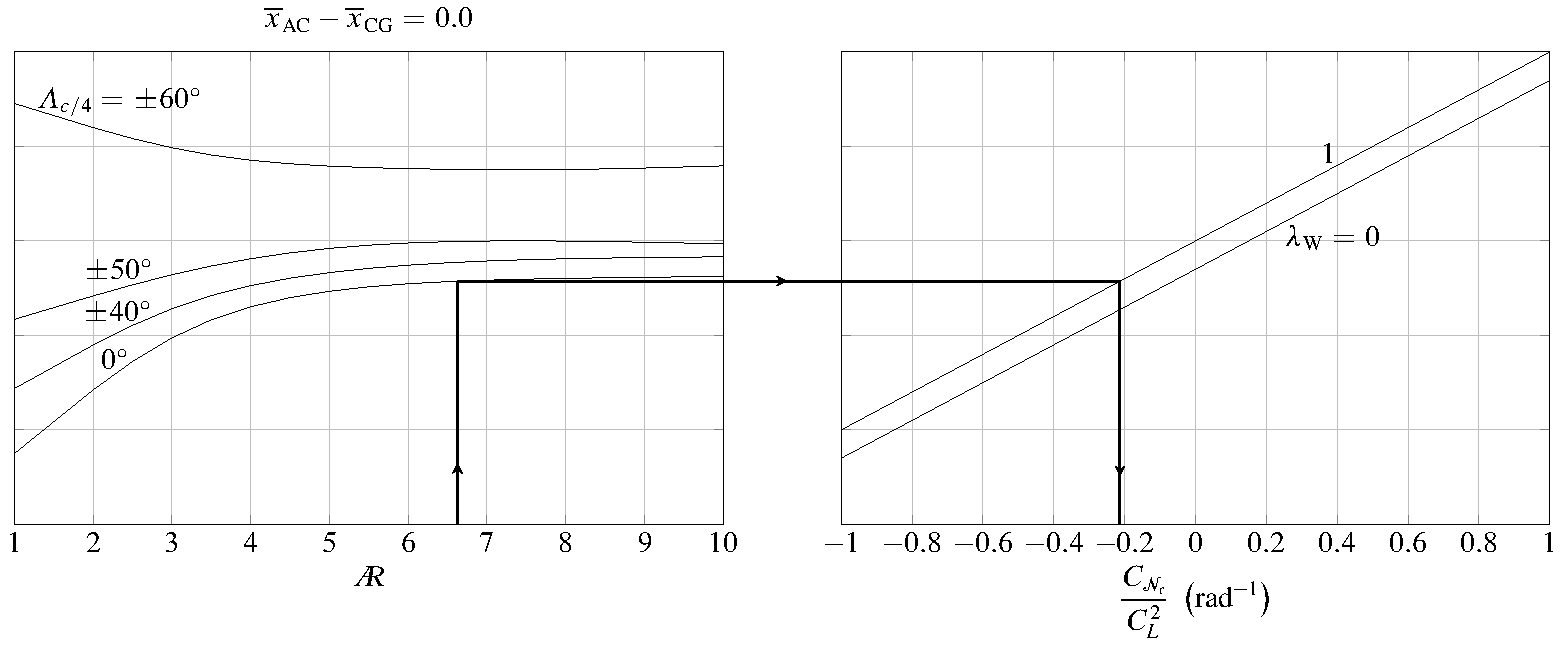
\includegraphics[width=\textwidth]{Immagini/Capitolo2/4_89-CNL_0}} \\
\subfloat[]
	{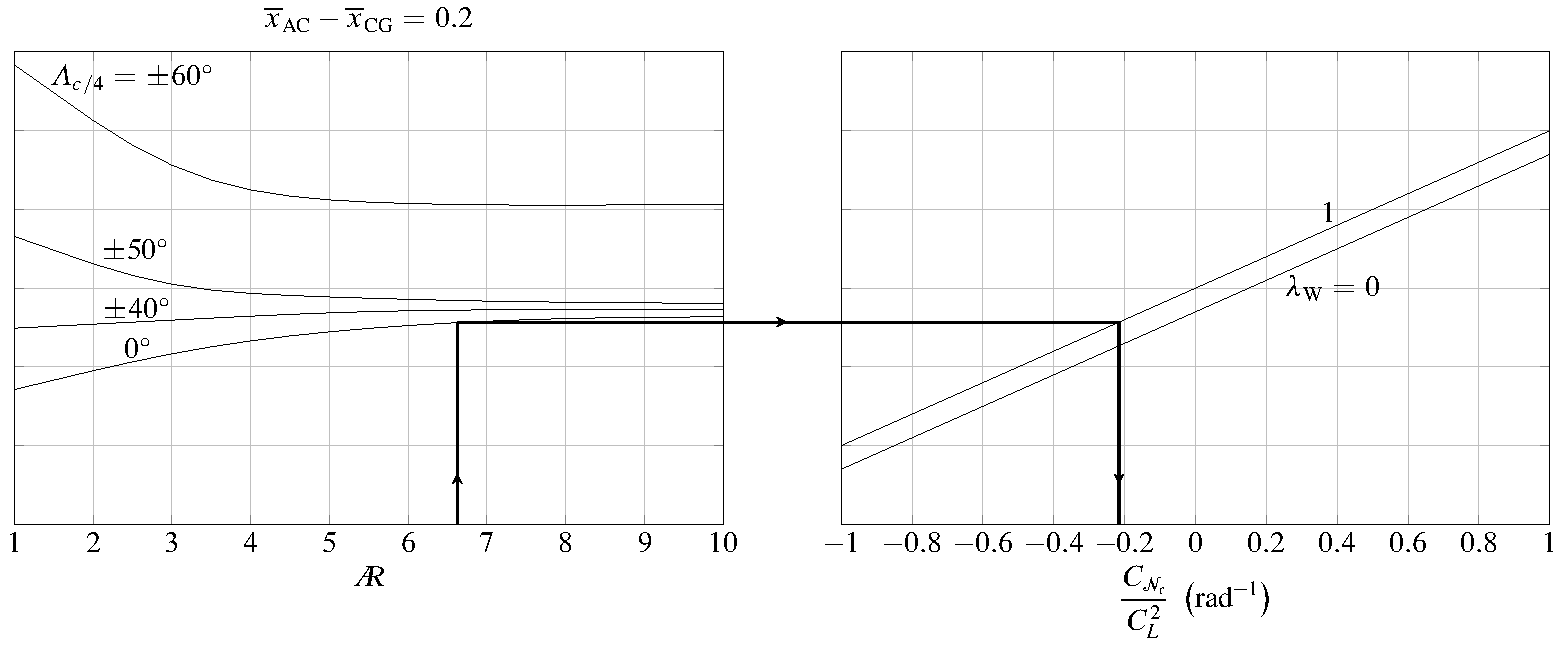
\includegraphics[width=\textwidth]{Immagini/Capitolo2/4_89-CNL_02}} \\
\subfloat[]
	{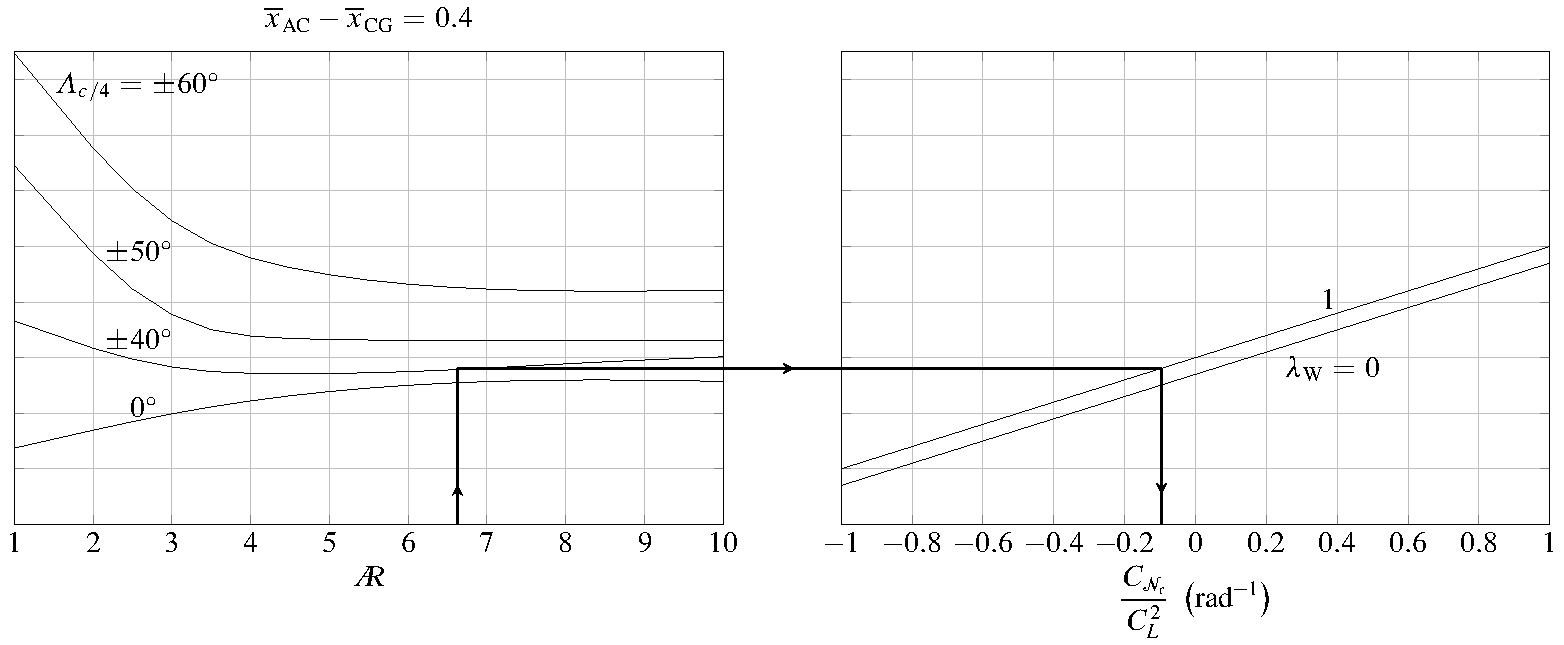
\includegraphics[width=\textwidth]{Immagini/Capitolo2/4_89-CNL_04}} \\
\caption[Evaluation of $C_{\mathcal N_\mathrm r}/C^2_L$ ] {Effect of lift on $C_{\mathcal N_r}$}
\label{CNR}
\end{figure}

\begin{figure}[htbp]
\centering
\subfloat[]
	{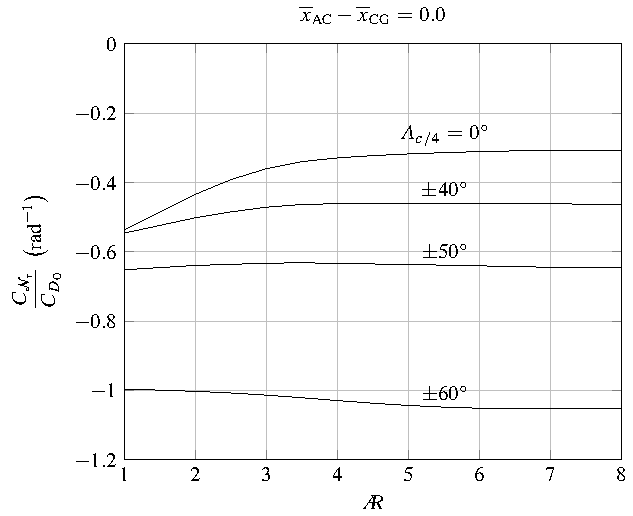
\includegraphics[width=.55\textwidth]{Immagini/Capitolo2/4_90-CND_0}} \\
\subfloat[]
	{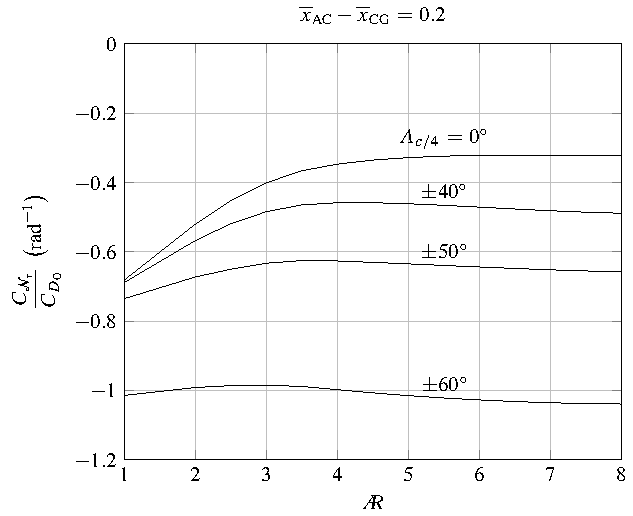
\includegraphics[width=.55\textwidth]{Immagini/Capitolo2/4_90-CND_02}} \\
\subfloat[]
	{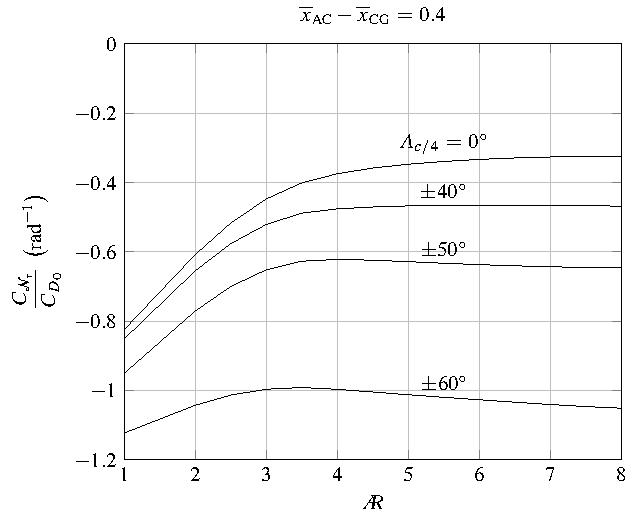
\includegraphics[width=.55\textwidth]{Immagini/Capitolo2/4_90-CND_04}}
\caption[Effect of $C_{D_0}$ on $C_{\mathcal N_\mathrm r}$] {Effect of parasite drag on $C_{\mathcal N_r}$}
\label{CND}
\end{figure}